\chapter{Conclusions and Future Perspectives}  \label{ch:conclusion}
\graphicspath{{conclusions/figures/}}

In this chapter, we summarize the major achievements of this thesis and we give an outlook on future perspectives.

\section{Scenario Flashback}

Going back to our scenario defined in Section~\ref{section:scenario}, we have defined two main personae. The first is a data analyst called \textbf{Dan} who works with the Ministry of Transport in France. He receives a memo from his management to create a report comparing the number of car accidents that occurred in France for this year, to its counterpart in the United Kingdom (UK). In addition, he is asked to highlight accidents related to illegal consumption of alcohol in both countries.

The second is a data portal administrator called \textbf{Paul}. He is affiliated with the British Open Data portal (\texttt{data.gov.uk}). His daily job includes acquiring, preparing and publishing relevant datasets on the portal. He always strives to maintain a spam-free, high-quality portal.

\section{Achievements}

This thesis thoroughly describes the different steps aiming at realizing the vision of enabling self service data provisioning in the enterprise (see Figure~\ref{fig:architecutre_diagram_annotated}). The work presented is beneficial to both our personae introduced. The contributions made are:

\begin{adjustwidth}{-.4in}{-.4in}
	\begin{figure}[!ht]
	  \centering
	  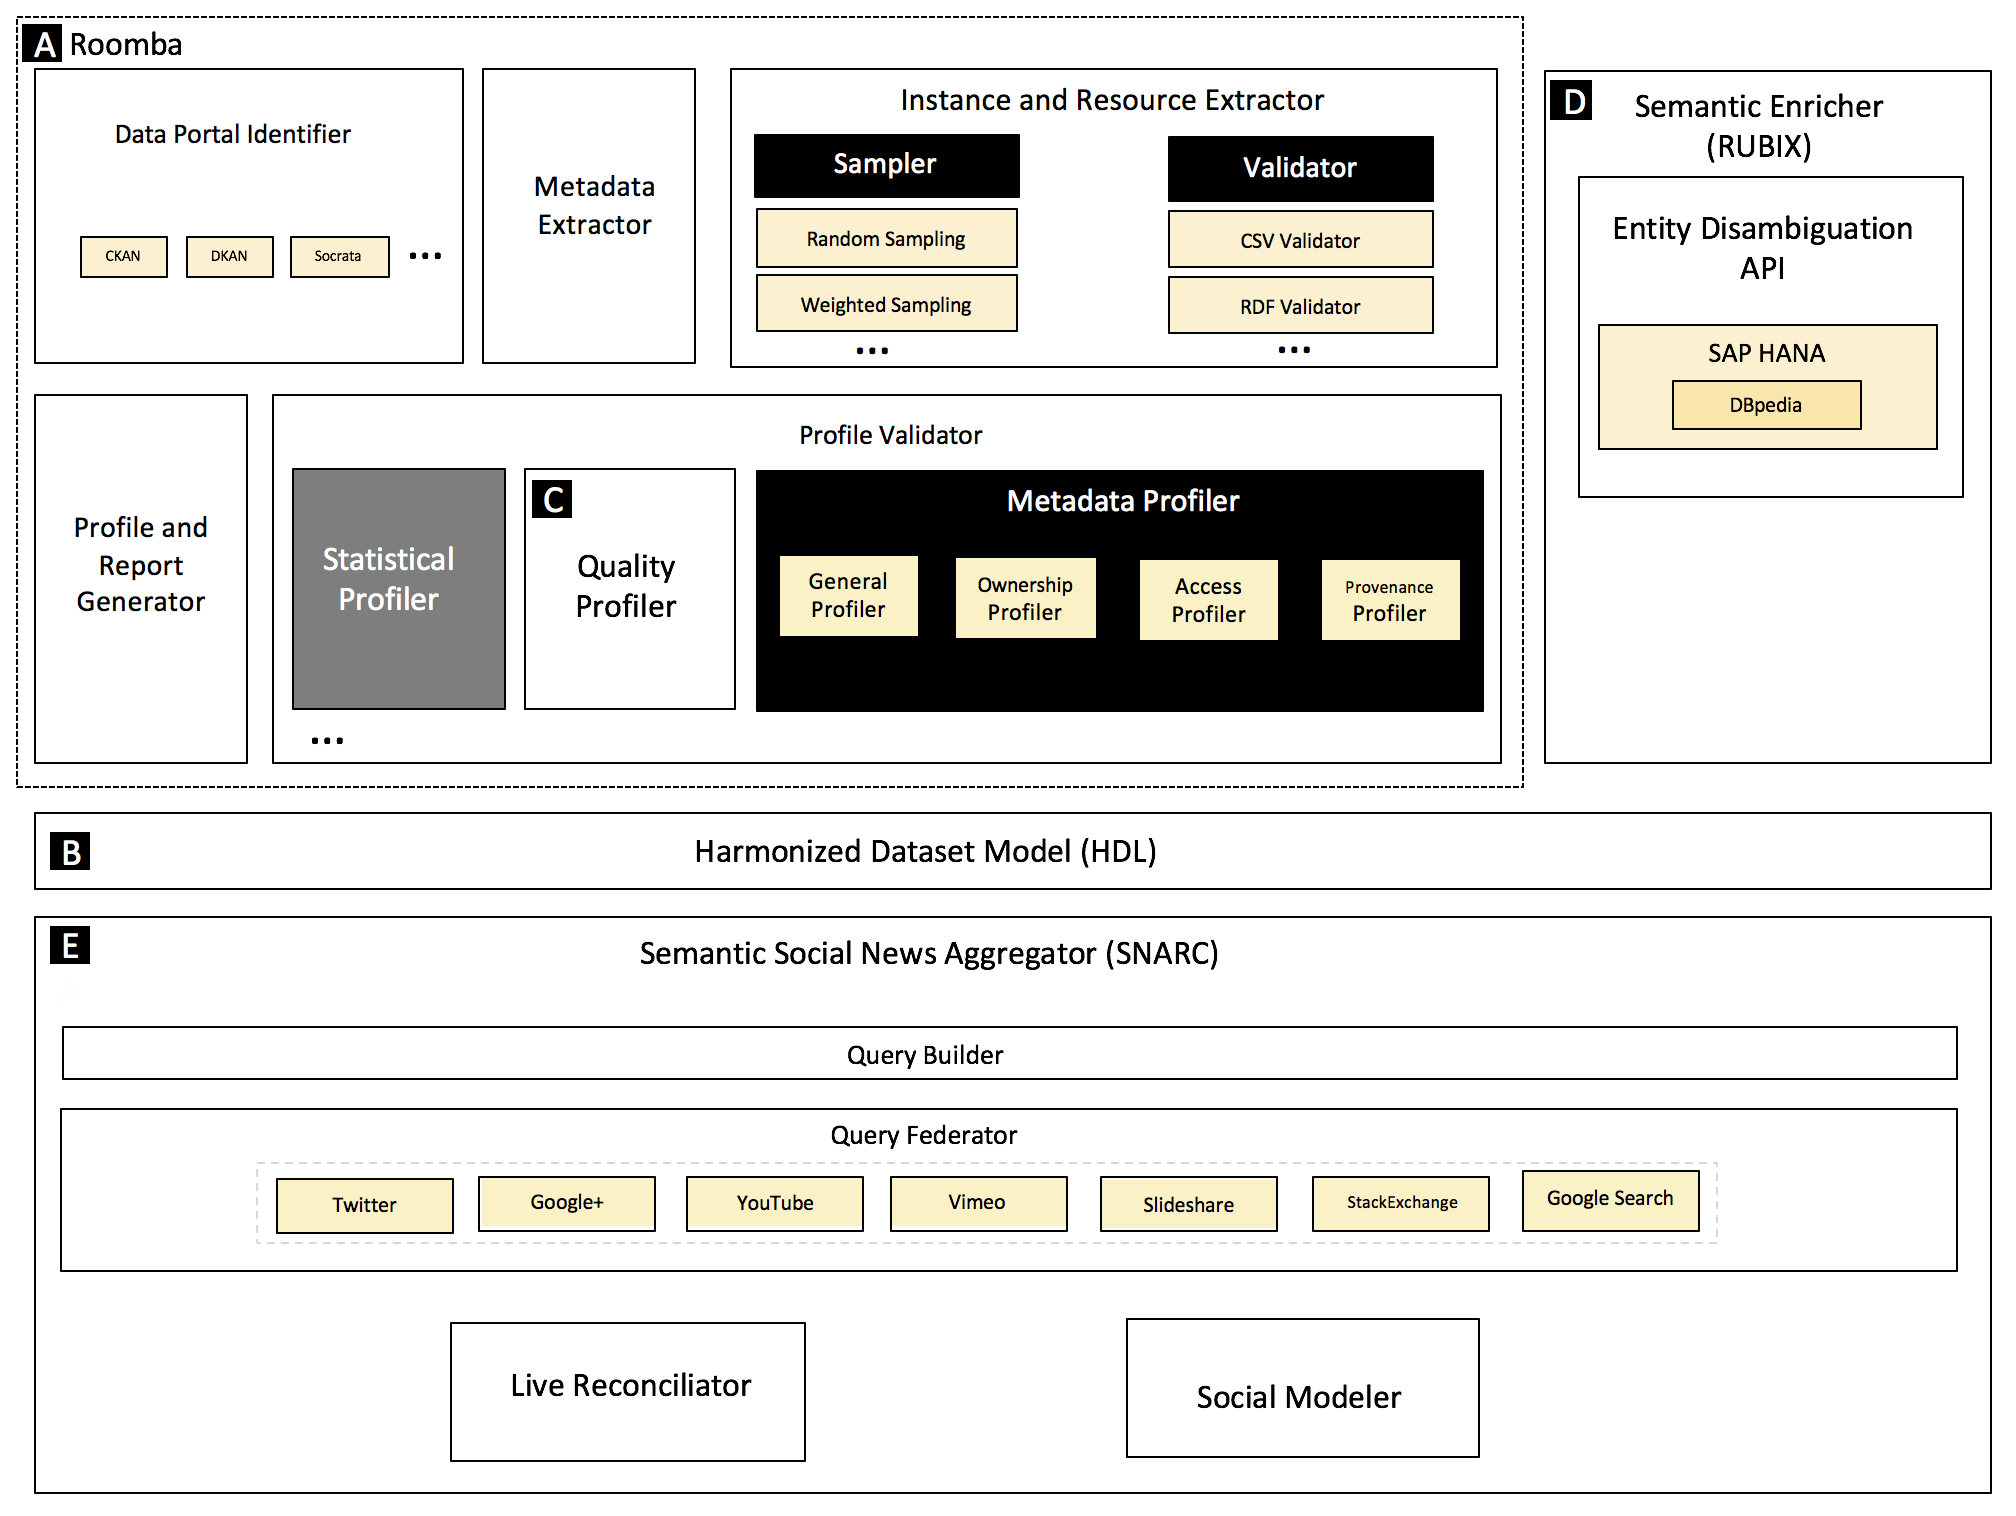
\includegraphics[scale=0.4]{architecutre_diagram_annotated.png}
	  \caption{Annoteted architecture diagram for enabling self-service data provisioning}
	  \label{fig:architecutre_diagram_annotated}
	\end{figure}
\end{adjustwidth}

\textbf{Contributions for Data Portals Administrators}
\vspace{1mm}
\\

Our data portal administrator \textbf{Paul} is always looking to expand his portals in terms of the number of datasets hosted, without compromising in their portal's data quality. In Chapter~\ref{chapter:hdl} (component \textbf{B} in Figure~\ref{fig:architecutre_diagram_annotated}), we surveyed the landscape of various models and vocabularies that described datasets on the web. We found a shortcoming when it comes to having a complete descriptive dataset model taking into account access, license and provenance information. As a result, we proposed a Harmonized Dataset Model (HDL) that \textbf{Paul} will use as a basis to extend and present the datasets he controls. \textbf{Paul} now also knows what are the major dataset models out there, and what kind of metadata data owners need to fully represent their dataset. The mappings proposed in Section~\ref{section:model_mappings} will allow him to easily integrate data from various data management systems into his own.

In Chapter~\ref{chapter:roomba} (component \textbf{A} in Figure~\ref{fig:architecutre_diagram_annotated}), we proposed Roomba, an automatic dataset profiles generation and validation tool that can be easily extended to perform various profiling tasks. Out of the box, \textbf{Paul} can use Roomba to automatically fix datasets metadata issues, and notify the datasets owners of the other issues to be manually fixed.

In Chapter~\ref{chapter:data-quality} (component \textbf{C} in Figure~\ref{fig:architecutre_diagram_annotated}), we proposed a comprehensive objective quality framework applied to the Linked Open Data. Moreover, after surveying the landscape of existing data quality tools, we identified several gaps and the need for a comprehensive evaluation and assessment framework and specifically for measuring quality on the dataset level. As a result, we presented an extension of Roomba that covers 82\% of the suggested datasets objective quality indicators. \textbf{Paul} will be able now to identify spam and low quality datasets. In addition to that, data available in his portal will now have rich semantic information attached to it. For example, temporal and spatial information extracted will be assigned into the corresponding fields in HDL. As an exemplary result, various datasets will be easily identifiable to cover various parts of the UK.\\

\textbf{Contributions for Data Analysts}
\vspace{1mm}\\

Our data analyst \textbf{Dan} believes that ``more data beats better algorithms'' and is always hunting for high quality data to produce accurate reports to the management team. By examining the rich datasets metadata presented in HDL he will be able to make fast decisions whether the dataset examined is suitable or not. He will also have vital information about the licensing and limitations for using this data internally. He will also have assurances on the dataset quality, which will help choose the best candidates out of ranked list.

\begin{wrapfigure}{r}{0.5\textwidth}
  \begin{center}
    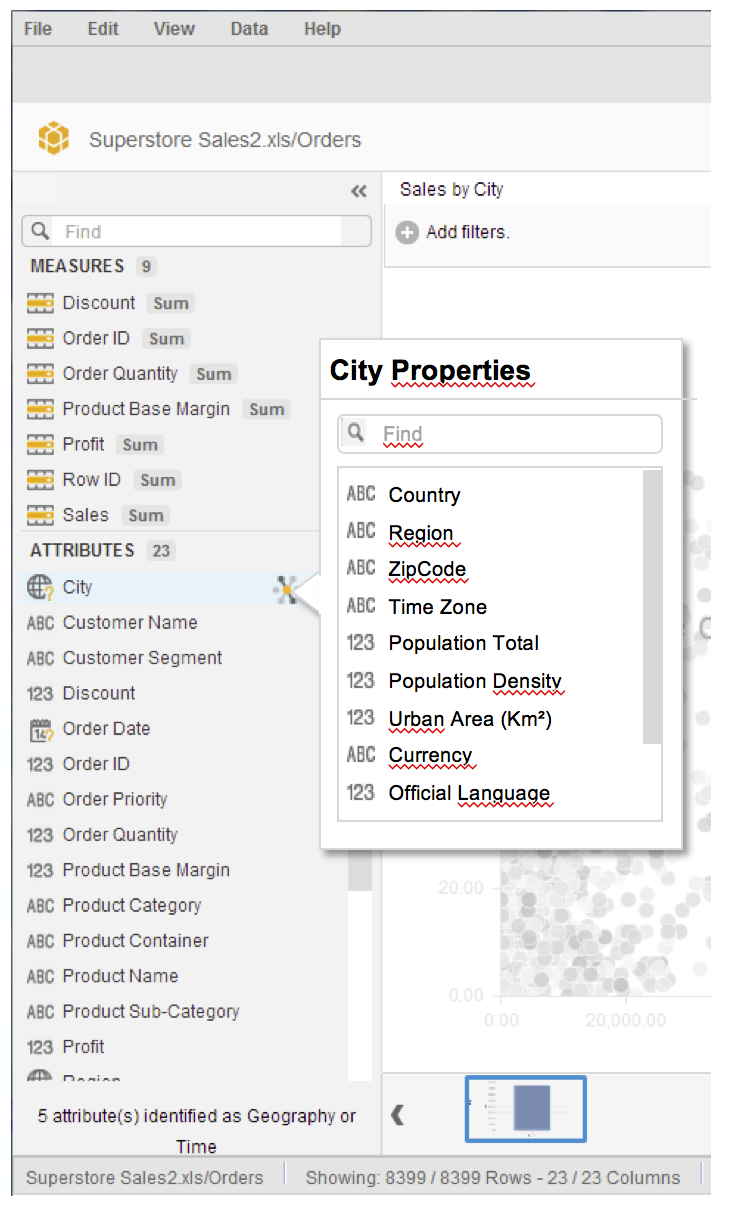
\includegraphics[width=0.48\textwidth]{lumira_sample.png}
  \end{center}
  \caption{UI Prototype of semantic data enrichment in SAP Lumira}
  \label{fig:lumira}
\end{wrapfigure}

\textbf{Dan} will be able to have direct access to rich and high-quality dataset descriptions generated by Roomba. Moreover, the topical profilers in Roomba will be able to identify occurrences of alcohol related terms like ``wine'' in various datasets. Query expansion methods can be used to relate alcohol to wine allowing him to find the datasets he wants.

In Chapter~\ref{chapter:rubix} (component \textbf{D} in Figure~\ref{fig:architecutre_diagram_annotated}), we presented an entity disambiguation API built on top of SAP HANA. This API is used in RUBIX, a framework we proposed to enable mashup of potentially noisy enterprise and external data.
\textbf{Dan} now has access to various datasets that he found matching his query to the portal administered by \textbf{Paul}. He will be also able to use the schema matching services to find and merge those datasets in his reports.

Having imported those dataset into Lumira, he will be also able to use the internal knowledge base to apply various semantic enrichments on this data. Figure~\ref{fig:lumira} shows a possible integration of such service in SAP Lumira where \textbf{Dan} is presented with a ranked set of properties retrieved by the algorithm proposed in Section~\ref{Section:EKG}.

In Chapter~\ref{chapter:snarc} (component \textbf{E} in Figure~\ref{fig:architecutre_diagram_annotated}), we proposed SNARC, a semantic social news aggregation service that allows the user to explore relevant news from internal or external sources. \textbf{Dan} is also a modern person, who is always trying to fresh information and believes in the wisdom of the crowd. Having SNARC services integrated with Lumira, he is also able to see a feed of relevant social media items that can be of interest to him. He actually follows a link in some tweet that he saw and was able to find relevant pieces of pointers that he would like to investigate further.

In summary, the contributions above pave the way to build a set of smart services to enable analysts easily find relevant pieces of information and administrators fight spam and be able to maintain high quality data portals. The work presented in this thesis goes beyond the fact that attaching metadata to datasets is vital, but propose a set of services that can automatically achieve that in seamless manner.

\section{Perspectives}

This thesis could be extended in the following directions:

\begin{itemize}

\item \textbf{Data Profile Representation}
\vspace{1mm}
\\
The proposed Harmonized Dataset Model (HDL) is currently available as a hierarchical JSON file. An enhancement would be to refine HDL and present it as a fully fledged OWL ontology. In addition, HDL can be extended to propose also a set of enumerations as values to ensure a unified fine-grained representation of a dataset. Moreover, while we presented the mappings between various models in a table structure, presenting those mappings in a machine readable format will allow various tools like Roomba to use it.

\item \textbf{Automatic Dataset Profiling}
\vspace{1mm}
\\
It has been noticed that the issues surrounding metadata quality affect directly dataset search as data portals rely on such information to power their search index. There are various extensions to our tool Roomba that can help in automatically building and enhancing dataset profiles. An example of these extension would be the integration of statistical and topical profilers allowing the generation of full comprehensive profiles. We would also like to extend Roomba to be able to run over other data portal types like DKAN or Socrata. This extension can be done by leveraging the data models mappings we proposed. In addition to all that, a possible enhancement will be ability to correct the rest of the metadata either automatically or through intuitive manually-driven interfaces.

\item \textbf{Objective Linked Data Quality}
\vspace{1mm}
\\
Ensuring data quality in Linked Open Data is a complex process as it consists of structured information supported by models, ontologies and vocabularies and contains queryable endpoints and links. In this thesis, we managed to narrow down the set of quality issues surrounding Linked Data to those who can be objectively measured and assessed by automatic tools. Our proposed tool covers 85\% of the quality indicators proposed. A possible extension would be to integrate tools assessing models quality in addition to syntactic checkers with Roomba. This will provide a complete coverage of the proposed quality indicators. Moreover, there are currently no weights assigned to the quality indicators. A valid contribution would be to suggest weights to those indicators which will result in a more objective quality calculation process.

\item \textbf{Enterprise Data Integration}
\vspace{1mm}
\\
A vital component to Data Integration in the enterprise is the existence of enterprise knowledge bases. Integrating additional linked open data sources of semantic types such as YAGO and evaluate our matching results against instance-based ontology alignment benchmarks such as OAEI\footnote{http://oaei.ontologymatching.org/2011/instance/index.html} or ISLab\footnote{http://islab.dico.unimi.it/iimb/} are possible future directions. Moreover, our work can be generalized to data classification. The same way the AMC helps identifying the best matches for two datasets, we plan to use it for identifying the best statistical classifiers for a sole dataset, based on normalized scores.
\end{itemize}